\chapter{Desarrollo e Implementación}

\section{Hardware}

El hardware se diseña por medio del software Proteus ...

\section{Firmware}

El firmware se desarrolla sobre el framework o SDK oficial de Espressif Systems, ESP-IDF el cual posee una documentación \cite{ES}, la cuál es muy útil a la hora de utilizar las diferentes APIs que este posee.\\

Sobre el firmware se desarrollan los siguientes temas:

\subsubsection{Consola}

Se usa para hacer pequeñas pruebas por medio de la construcción de comandos ligados a funciones ...

\subsubsection{HTTP Request}

Para realizar las diferentes peticiones de HTTP se utiliza la libreria lwip ...

\subsubsection{Tareas}

Las tareas son funciones propias de los sistemas operativos en tiempo real ...

\subsubsection{Timers}

Son utilizados principalmente para el control de cargas AC ...

\subsubsection{I2C}

El protocolo I2C se activa por medio de la instalación del driver en algún par de pines ...

\subsubsection{PWM}

Se usan para el control de cargas DC ...

\subsubsection{GPIO}

El ESP-WROOM-32 posee diferentes GPIO, los cuales se usan para leer o escribir señales digitales a los sensores o ...

\subsubsection{Interrupciones}

Las interrupciones se usan para no gastar recursos en un monitoreo constante de las entradas, solo cuando exista un cambio de nivel en la entrada el dispositivo desencadena una serie de instrucciones ...

\section{Software}

Para el software se utiliza una plataforma como servicio (Pass) el cuál es el servicio que ofrece la plataforma Heroku, en este caso se usa una cuenta gratuita para realizar las pruebas de la aplicación, allí en el servidor de la plataforma se aloja la aplicación desarrollada en HTML5 y PHP.\\

Por este motivo se usa el framework Laravel, el cual como se menciona anteriormente combina HTML5, PHP y un ORM, para realizar el manejo de toda la parte del servidor se usa PHP, este framework proporciona un mapeo de consultas para las bases de datos, así que las consultas se hacen como codigo de PHP y este se encarga de realizar los comando de SQL necesarios, lo que facilita que la aplicación use diferentes gestores de bases de datos como MySQL, SQLite, entre otras.\\

Para el software se toman en cuenta dos tipos de vista, una vista pública y una privada, como se observa en la figura \ref{fig:index}. En la vista pública se encuentran los datos generados por los sensores, agrupados por el tipo de variable que estan midiendo, temperatura, humedad, entre otras. En la vista privada se encuentra la interacción de los usuarios y dueños de las casas, para controlar y ver sus datos.\\

\begin{figure}
	\centering
	\caption{Página de Inicio}
	\label{fig:index}
	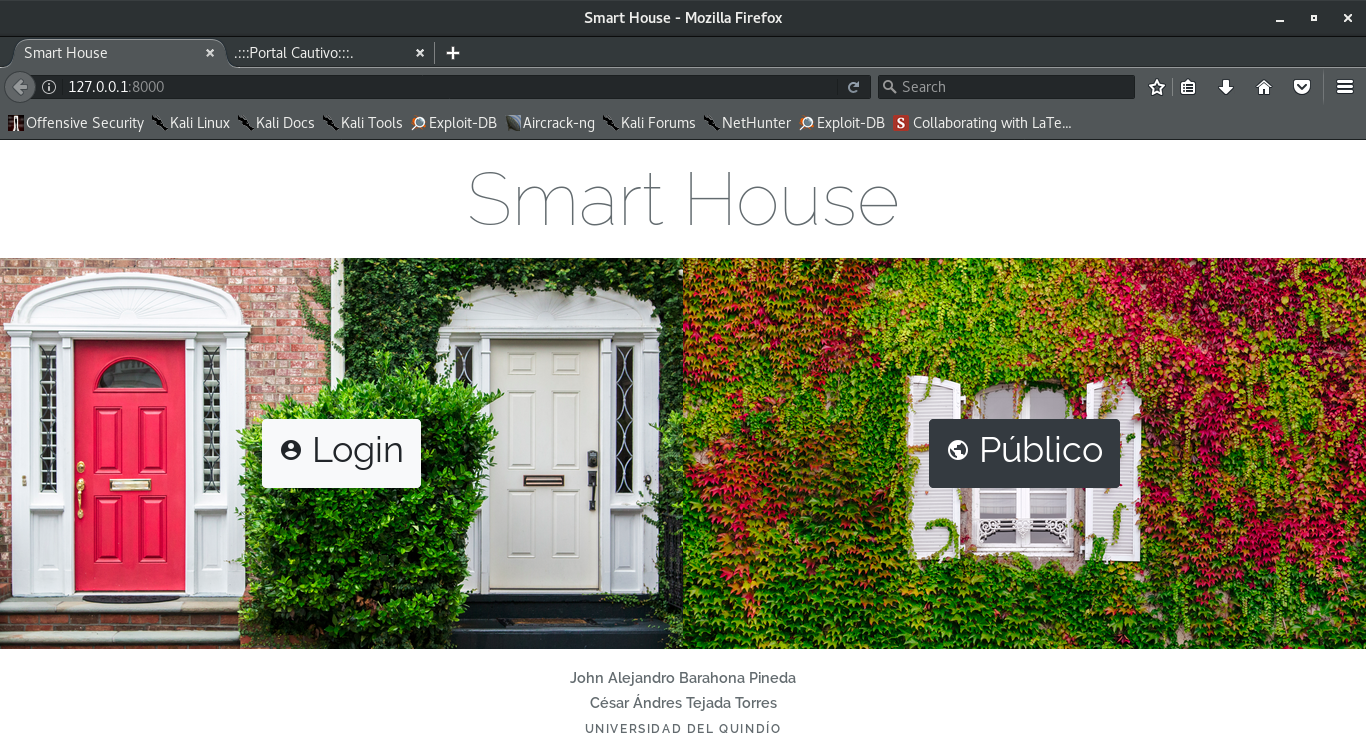
\includegraphics[width=0.9\linewidth]{Imagenes/Index}
\end{figure}


Esta parte se garantiza por medio del framework, creando diferentes roles para cada usuario que se esta registrando y realizando la comprobación por parte del Middleware que provee este.\\

Para el manejo de los diferentes sensores y usuarios todo se registra en la base de datos que facilita la plataforma Heroku.\\

\subsection{Parte Pública}

En esta vista se encuentran los datos sin etiquetas que identifiquen la procedencia de estos, solamente se pueden observar los historicos de las variables medidas.\\

IMAGEN DE LA VISTA

\subsection{Parte Privada}

En esta sección es donde se encuentra el Panel de Control para un usuario administrador que son los dueños de la apliación, usuarios dueños de las diferentes casas que poseen el dispositivo y otro usuario dueño de la habitación donde se encuentra el dispositivo, este ultimo usuario está sujeto a un usuario dueño de la casa, ya que el usuario de la casa puede gestionar todas las habitaciones mientras que el usuario de habitación solamente le compete su habitación.\\

IMAGEN DE LA VISTA ADMIN\\

IMG VISTA CASA\\

IMG VISTA CUARTO\\

\subsection{Base de Datos}

En la base de datos se crean las siguientes tablas, para guardar la información pertinente, se crea una tabla de usuarios, una tabla de sensores, de datos...\\

IMAGEN CON LAS TABLAS Y LAS RELACIONES
